% Copyright © 2017-2018 Martin Ueding <martin-ueding.de>
% Licensed under CC-BY 4.0

\documentclass{scrartcl}

\pagestyle{empty}

\usepackage{tikz}
\usetikzlibrary{arrows.meta, calc}

\colorlet{mygray1}{black!10}
\colorlet{mygray2}{black!20}

\begin{document}

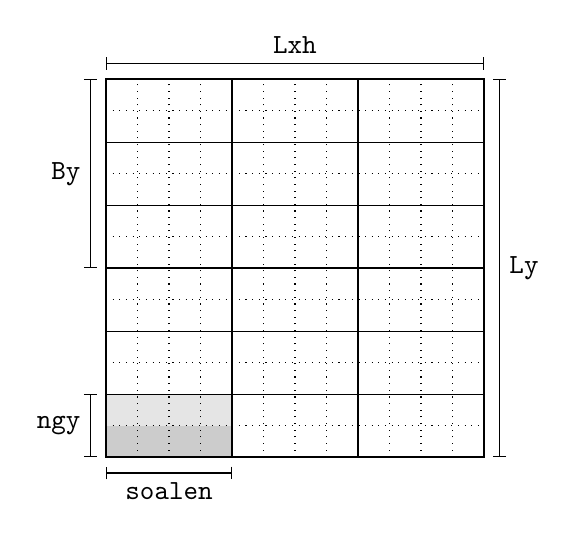
\begin{tikzpicture}[scale=0.4]

    \fill[fill=mygray2] (0, 0) rectangle +(4, 1);
    \fill[fill=mygray1] (0, 1) rectangle +(4, 1);

    \draw[thick, xstep=4, ystep=6] (0, 0) grid (12, 12);
    \draw[thick] (0, 0) rectangle (12, 12);

    \draw[thin, xstep=4, ystep=2] (0, 0) grid (12, 12);
    \draw[dotted] (0, 0) grid (12, 12);

    \draw[|-|] (0, -0.5) -- (4, -0.5) node[below, midway] {\texttt{soalen}};
    \draw[|-|] (-0.5, 0) -- (-0.5, 2) node[left, midway] {\texttt{ngy}};
    \draw[|-|] (-0.5, 6) -- (-0.5, 12) node[left, midway] {\texttt{By}};
    \draw[|-|] (12.5, 0) -- (12.5, 12) node[right, midway] {\texttt{Ly}};
    \draw[|-|] (0, 12.5) -- (12, 12.5) node[above, midway] {\texttt{Lxh}};

\end{tikzpicture}

\end{document}
